
\documentclass[12pt]{article}
\pagestyle{empty} \topmargin -0.5in \textheight 9in \textwidth 6.5in
\oddsidemargin -0in
\usepackage{amssymb}
\usepackage{amsmath}
\usepackage{xcolor}
\usepackage{graphicx}
\usepackage[normalem]{ulem}
\usepackage{enumerate}

\DeclareMathOperator{\tr}{tr}

\newcommand{\vect}[1]{\mathbf{#1}}

\begin{document}

\textcolor{blue}{Andrew Yonan (10973951)}
\begin{flushleft}

\textbf{Department of Applied Mathematics and Statistics}

\textbf{COLORADO SCHOOL OF MINES}\\


MATH $455$: Partial Differential Equations
\end{flushleft}

\vspace{0.1in}

\begin{center}
{\bf Assignment \#2 - More Fourier Series} \\
Due Thursday, September 17, 2026 \\
\end{center}

\vspace{0.3in}

\noindent $\textbf{1}$. (12 points) Define the function
$$f(x) =
\begin{cases}
	1, & \mathrm{if} \ |x| < \frac{\pi}{2} \\ 
	0, & \mathrm{if} \ |x| > \frac{\pi}{2},
\end{cases}$$
and let $F(x)$ be the Fourier series of $f(x)$ on the interval $(-\pi, \pi)$. Sketch by hand $F(x)$ on the interval $(-3\pi, 3\pi)$ and compute a formula for $F(x)$ using the Fourier coefficients. \\

\textcolor{blue}{\textbf{Solution} — Since $f$ is not periodic on $\mathbb{R}$, we restrict its domain to $[-\pi, \pi]$ and fill in left-right-averaged discontinuities: 
$$f_{2\pi}(x) =
\begin{cases}
	1 & \mathrm{if} \;\; |x| < \frac{\pi}{2} \\ 
	0 &  \mathrm{if} \;\;  \frac{\pi}{2} < |x| \leq \pi \\
	\frac{1}{2} & \mathrm{if} \;\; |x| = \frac{\pi}{2} \\
\end{cases}$$ \\ Now let $g(x)$ be the periodic extension of $f_{2\pi}(x)$ to all $\mathbb{R}$. By the Fourier convergence theorem, $F(x) = g(x)$ for all $\mathbb{R}$, so sketching $F(x)$ on $(-3\pi, 3\pi)$  is equivalent to sketching $g(x)$ on $(-3\pi, 3\pi)$: \\ 
\begin{figure}[h]
    \centering 
    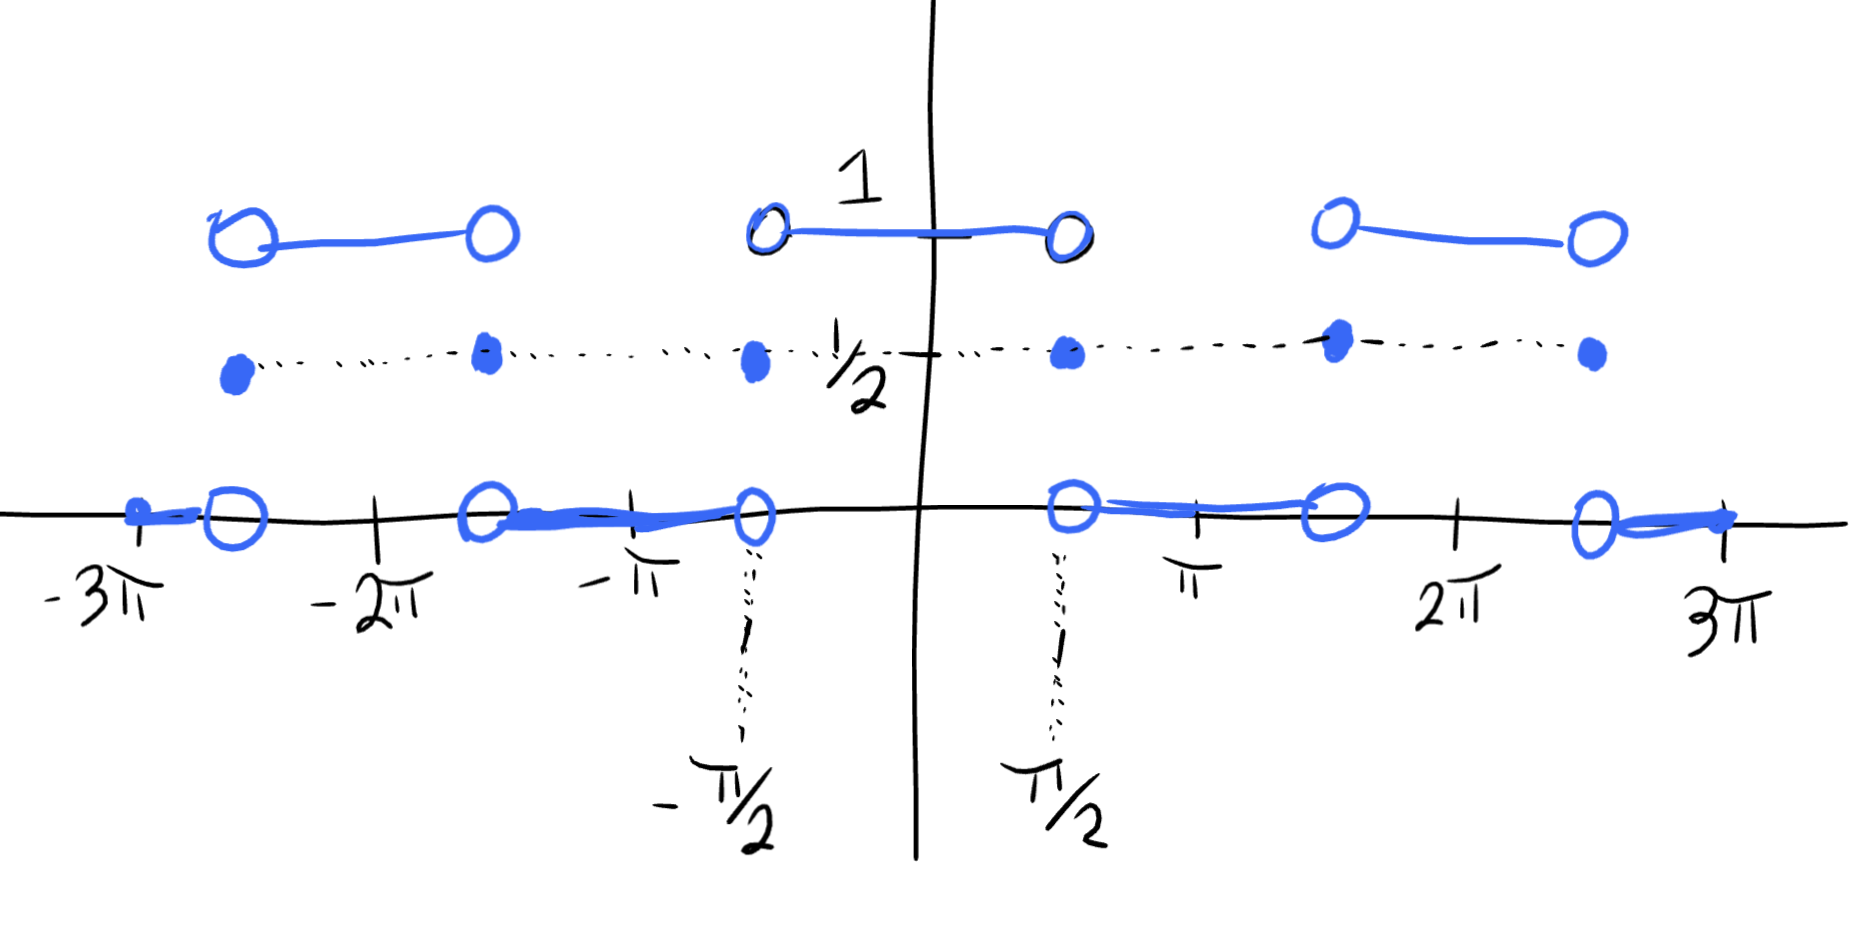
\includegraphics[width=0.5\textwidth]{Q1}
\end{figure} \\
We compute the Fourier series of $g(x)$: \\ 
\begin{align*}
a_0 &= \frac{1}{\pi} \int_{-\pi}^{\pi} g(x) dx = 1 \\
b_n &= \frac{1}{\pi} \int_{-\pi}^{\pi} g(x) \sin(nx) dx = 0 \;\;\; \text{(by oddness of product $g(x)\sin(nx)$)} \\
a_n &= \frac{1}{\pi} \int_{-\pi}^{\pi} g(x) \cos(nx) dx \\
&= \frac{1}{\pi} \int_{-\pi/2}^{\pi/2} \cos(nx) dx \\
&= \frac{1}{\pi} \left[ \frac{1}{n} \sin(nx)  |_{-\pi/2}^{\pi/2} \right] \\
&= \frac{2}{n\pi}  \sin \left( \frac{n\pi}{2} \right)  \\
\end{align*}
Hence 
\begin{align*}
F(x) &= \frac{1}{2} + \sum_{n=0}^{\infty} \left[ \frac{2}{n\pi} \sin \left( \frac{n\pi}{2} \right)  \right] \cos(nx) \\
&= \frac{1}{2} + \frac{2}{\pi}\sum_{n=0}^{\infty} \left[ \frac{1}{n} \sin \left( \frac{n\pi}{2} \right)  \right] \cos(nx) \\
\end{align*}
Since
$$\sin \left( \frac{n\pi}{2} \right) = \begin{cases}
	0 & \mathrm{if} \;\; n \;\; \text{even} \\ 
	1 &  \mathrm{if} \;\;  n \equiv 1 \mod(4)\\
	-1 & \mathrm{if} \;\; n \equiv 3 \mod (4) \\
\end{cases}$$
we want to skip the even terms, hopping over the odd terms instead, and alternating between a $1$ and $-1$ coefficient, starting with $1$:
\begin{align*}
F(x) &= \frac{1}{2} + \frac{2}{\pi}\sum_{n=0}^{\infty} \frac{(-1)^n}{2n+1} \cos((2n+1)x) \\
\end{align*}
}

\vspace{0.3in}

\noindent $\textbf{2}$. (8 points) We know that if $f(x)$ is odd on the interval $(-\pi, \pi)$, then its Fourier series is composed of only sine functions. What additional symmetry condition on $f$ will make the sine coefficients with even indices become zero (i.e., $b_{2n} = 0 $ for all $n \in \mathbb{Z}$)? Provide a specific example of a function with this property and show that it satisfies the condition. \\

\textcolor{blue}{\textbf{Solution —} Let $f(x)$ be odd. We want to find additional conditions on $f(x)$ that will force $b_{n} = 0$ for even $n$, or equivalently, to force $b_{2n} = 0$ for all $n$:
\begin{align*}
b_{2n} &= \frac{1}{\pi} \int_{-\pi}^{\pi} f(x) \sin(2nx) dx = 0 \\
&= \frac{2}{\pi} \int_{0}^{\pi} f(x) \sin(2nx) dx \;\;\; \text{(by evenness of $f(x)\sin(2nx)$)} \\
\end{align*}
Note that $\sin(2nx)$ is odd about $x=\frac{\pi}{2}$: 
\begin{align*}
& \sin\left( 2n \left( \frac{\pi}{2} + h \right) \right) \\
&= \sin\left( n\pi + 2nh \right) \\
&= \sin(n\pi) \cos(2nh) + \cos(n\pi)\sin(2nh)\\
&= -(\sin(n\pi) \cos(2nh) - \cos(n\pi)\sin(2nh))\\
&= -\sin\left( n\pi - 2nh \right) \\
&= - \sin\left( 2n \left( \frac{\pi}{2} - h \right) \right)
\end{align*}
$x = \frac{\pi}{2}$ is the midpoint of our integration range $[0, \pi]$, so the $[0, \pi]$-integral of any function that is odd about $x=\frac{\pi}{2}$ must be zero. Hence, for $\int_{0}^{\pi} f(x)\sin(2nx)dx$ to be zero, we require $f(x)$ to be even about $x = \frac{\pi}{2}$. \\ \\
One such function is $f(x) = (x - \frac{\pi}{2})^2$ \\ \\ This function satisfies evenness about $\frac{\pi}{2}$:
\begin{align*}
f\left( \frac{\pi}{2} - h \right) &= \left( \left( \frac{\pi}{2}-h \right) - \frac{\pi}{2} \right)^2 \\
&= (-h)^2 \\
&= (h)^2 \\
&= \left( \frac{\pi}{2} + h - \frac{\pi}{2} \right)^2\\
&= \left( \left( \frac{\pi}{2} + h \right) - \frac{\pi}{2} \right)^2\\
&= f\left( \frac{\pi}{2} + h \right) \\
\end{align*}
}

\vspace{0.3in}


\noindent $\textbf{3}$. (12 points) Let 
$$f(x) = x\cos(x), \quad x \in \left (-\frac{\pi}{2},\frac{\pi}{2} \right )$$
$$g(x) = x\cos(x), \quad x \in (-1,1),$$
and
$$h(x) =
\begin{cases}
	0, & \mathrm{if} \ 1 < x < 3 \\ 
	1, & \mathrm{if} \ -1 < x < 1 \\ 
	x, & \mathrm{if} \ -3 < x < -1
\end{cases}$$
be periodic functions (defined via periodic extension) for $x \in \mathbb{R}$.
For each function
\begin{enumerate}[(a)]
\item Determine whether or not the function is in $\mathrm{PC}^1$ on the interval over which it is defined. \\  \\
\textcolor{blue}{\textbf{Solution —} A}
\item State the function to which its Fourier series (defined on the interval: $\left [-\frac{\pi}{2},\frac{\pi}{2} \right ]$ for $f(x)$, $[-1,1]$ for $g(x)$, and $[-3,3]$ for $h(x)$) converges\\
Note: Do not compute the Fourier series (or coefficients) to do this! \\ \\
\textcolor{blue}{\textbf{Solution —} A}
\item Sketch by hand three periods of the Fourier series in part (b). \\ \\ 
\textcolor{blue}{\textbf{Solution —} A}
\end{enumerate}


\vspace{0.3in}


\noindent $\textbf{4}$. (8 points) Let 
$$F(x) = \sum_{n=1}^\infty \frac{(-1)^n n^{3/2} + 2}{n^8 + 2n^6 + 1} \cos(nx)$$
How many continuous derivatives can we be sure that $F$
possesses? Justify your answer using tools from Calculus II. \\ \\
\textcolor{blue}{\textbf{Solution —} A}


\end{document}


